\section{Ekvipotensial sirtlar}

\begin{enumerate}

    \item Zaryadi 0,9 C bo‘lgan nuqtaviy zaryad kuchlanganligi 200 V/m bo‘lgan bir jinsli elektr maydonda kuch chiziqlariga nisbatan $53^\circ$ burchak ostida 30 cm ga ko‘chdi. Elektr maydonning bajargan ishini toping (J).
    \begin{enumerate}[label=\Alph*)]
        \item 108
        \item 120
        \item 180
        \item 100
        \item 90
    \end{enumerate}

    \item Maydonning E nuqtasidagi potensiali -8 V ga teng. Bu nuqtaga cheksiz uzoqlikdan kiritilgan 5 mC zaryadli zarra olgan potensial energiyani toping (mJ).
    \begin{enumerate}[label=\Alph*)]
        \item 40
        \item -40
        \item 1,6
        \item -1,6
        \item 0,625
    \end{enumerate}

    \item 4 $\mu$C zaryad kuchlanganligi bir jinsli elektrostatik maydonda rasmdagi kabi A nuqtadan B nuqtaga ko‘chirilganda 96 $\mu$J ish bajarilgan bo‘lsa, maydon kuchlanganligi moduli qanday (V/m)?

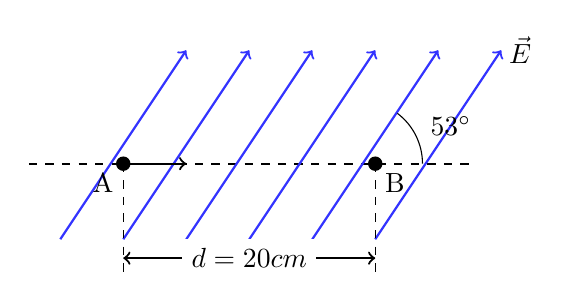
\begin{tikzpicture}[scale=0.8]
    % Gorizontal punktir chiziq
    \draw[dashed, thick] (-1,0) -- (6,0);

    % Elektr maydon chiziqlari (53 gradus burchak ostida parallel strelkalar)
    \foreach \x in {0,1,2,3,4,5} {
        \draw[->, thick, blue!80] (\x-0.5, -1.2) -- (\x+1.5, 1.8);
    }
    % Maydon kuchlanganligi belgisi
    \node at (6.8, 1.8) {$\vec{E}$};

    % A nuqta (zaryadlangan sharcha bilan)
    \filldraw (0.5,0) circle (3pt) node[below left] {A};
    % A nuqtadan yo'nalgan kichik tezlik/ko'chish strelkasi
    \draw[->, thick] (0.5,0) -- (1.5,0);

    % B nuqta
    \filldraw (4.5,0) circle (3pt) node[below right] {B};

    % 53 gradus burchakni ko'rsatish
    \draw (4.25,0) ++(0:1) arc (0:53:1);
    \node at (5.7,0.6) {$53^\circ$};

    % Masofani ko'rsatuvchi vertikal punktir chiziqlar
    \draw[dashed] (0.5,0) -- (0.5,-1.8);
    \draw[dashed] (4.5,0) -- (4.5,-1.8);

    % d=20 cm masofa ko'rsatkichi
    \draw[<->, thick] (0.5,-1.5) -- node[fill=white] {$d=20 \text{ cm}$} (4.5,-1.5);

\end{tikzpicture}
    
    \begin{enumerate}[label=\Alph*)]
        \item 900
        \item 600
        \item 450
        \item 300
        \item 200
    \end{enumerate}

    \item Elektrostatik maydonning potensiali 40 V bo‘lgan nuqtasidan potensiali –10 V bo‘lgan nuqtasiga $2 \cdot 10^{-7}$ C musbat zaryadni ko‘chirishda necha Joul ish bajariladi?
    \begin{enumerate}[label=\Alph*)]
        \item $2 \cdot 10^{-5}$
        \item $6 \cdot 10^{-6}$
        \item $1 \cdot 10^{-5}$
        \item $6 \cdot 10^{-7}$
        \item $1 \cdot 10^{-7}$
    \end{enumerate}

    \item Elektr maydon 1-nuqtadan 2-nuqtaga 1 C musbat zaryadni ko‘chirishda necha Joul ish bajaradi? Nuqtalar orasidagi potensiallar farqi 10 V.

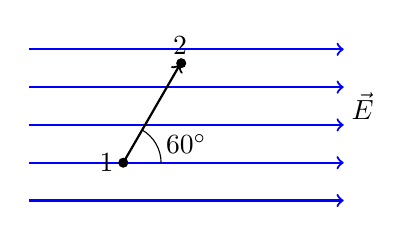
\begin{tikzpicture}[scale=0.8]
    % Elektr maydon chiziqlari (Gorizontal parallel strelkalar)
    \foreach \y in {0, 0.6, 1.2, 1.8, 2.4} {
        \draw[->, thick, blue] (-0.5, \y) -- (4.5, \y);
    }
    % Maydon kuchlanganligi belgisi
    \node at (4.8, 1.5) {$\vec{E}$};

    % Nuqtalarni belgilash (1-nuqta pastda, 2-nuqta yuqorida)
    \filldraw (1,0.6) circle (2pt);
    \filldraw (1.92,2.18) circle (2pt);
    \coordinate (P1) at (1, 0.6);
    \coordinate (P2) at ({1 + 1.8*cos(60)}, {0.6 + 1.8*sin(60)});

    % 1-nuqtadan 2-nuqtaga ko'chish chizig'i va yo'nalish strelkasi
    \draw[thick, ->] (P1) -- (P2);

    % Nuqta raqamlari
    \node[left] at (P1) {1};
    \node[above] at (P2) {2};

    % 60 gradus burchakni ko'rsatuvchi yoy
    \draw (1.6, 0.6) arc (0:60:0.6);
    \node at (2.0, 0.9) {$60^\circ$};

\end{tikzpicture}
    
    \begin{enumerate}[label=\Alph*)]
        \item 0
        \item 10
        \item 8,7
        \item 5
        \item 17
    \end{enumerate}

    \item $1,2 \cdot 10^{-4}$ C zaryadni bir nuqtadan ikkinchi nuqtaga ko‘chirishda 0,6 mJ ish bajarildi. Nuqtalar orasidagi potensiallar farqini aniqlang (V).
    \begin{enumerate}[label=\Alph*)]
        \item 10
        \item 5
        \item 3
        \item 0,7
        \item 0,5
    \end{enumerate}

    \item Elektronni elektr maydonda bir nuqtadan ikkinchi nuqtaga ko‘chirish natijasida uning kinetik energiyasi $8 \cdot 10^{-19}$ J ga o‘zgardi. Shu ikki nuqta orasidagi potensiallar farqini qanday (V). $e=1,6 \cdot 10^{-19}$ C.
    \begin{enumerate}[label=\Alph*)]
        \item 32
        \item 16
        \item 8
        \item 6
        \item 5
    \end{enumerate}

    \item Elektr maydonda elektronning tezligi $1 \cdot 10^7$ dan $5 \cdot 10^7$ m/s gacha oshdi. Boshlang‘ich va oxirgi nuqtalar orasidagi potensiallar ayirmasi qanday (kV)? Elektron zaryadining massasiga nisbati $1,76 \cdot 10^{11}$ C/kg.
    \begin{enumerate}[label=\Alph*)]
        \item 3,4
        \item 4
        \item 6
        \item 1,76
        \item 6,8
    \end{enumerate}

    
    \item Chizmada keltirilgan bir jinsli elektr maydondagi 2- va 3-nuqtalar orasidagi potensiallar farqi 6 V bo‘lsa, 1- va 3- nuqtalar orasida 3,5 $\mu$C zaryadni ko‘chirishda qanday ($\mu$J) ish bajariladi?

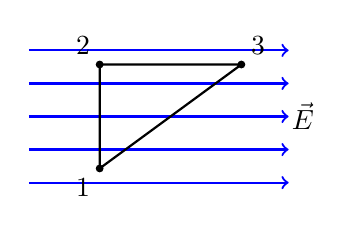
\begin{tikzpicture}[scale=0.6]
    % Elektr maydon chiziqlari (Gorizontal parallel strelkalar)
    \foreach \y in {0, 0.7, 1.4, 2.1, 2.8} {
        \draw[->, thick, blue] (-0.5, \y) -- (5, \y);
    }
    % Maydon kuchlanganligi belgisi
    \node at (5.3, 1.4) {$\vec{E}$};

    % Nuqtalarni belgilash (To'g'ri burchakli uchburchak)
    % 1-nuqta pastki chap burchakda
    % 2-nuqta 1 ning tepasida (vertikal)
    % 3-nuqta 2 ning o'ng tomonida (gorizontal)
    \coordinate (P1) at (1, 0.3);
    \coordinate (P2) at (1, 2.5);
    \coordinate (P3) at (4, 2.5);

    % Uchburchak chiziqlarini chizish
    \draw[thick] (P1) -- (P2) -- (P3) -- cycle;

    % Nuqtalarni kichik doira bilan belgilash
    \filldraw (P1) circle (2pt) node[below left] {1};
    \filldraw (P2) circle (2pt) node[above left] {2};
    \filldraw (P3) circle (2pt) node[above right] {3};

\end{tikzpicture}
    
    \begin{enumerate}[label=\Alph*)]
        \item 4
        \item $4\sqrt{2}$
        \item 21
        \item $8\sqrt{2}$
        \item 16
    \end{enumerate}

    \item Chizmada keltirilgan bir jinsli elektr maydondagi 1-, 2- va 3-nuqtalar teng tomonli uchburchakning uchlariga to‘g‘ri keladi. 1- va 3-nuqtalar orasidagi potensiallar farqi 16 V bo‘lsa, 2- va 3-nuqtalar orasida 2,5 $\mu$C zaryadni ko‘chirishda qanday ($\mu$J) ish bajariladi?

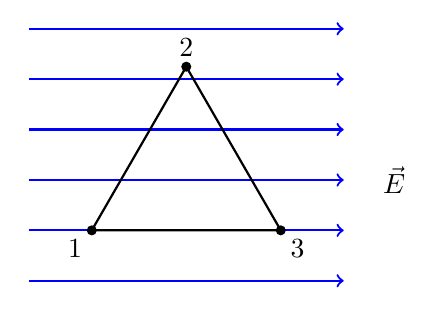
\begin{tikzpicture}[scale=0.8]
    % Elektr maydon chiziqlari (Gorizontal parallel strelkalar)
    \foreach \y in {0, 0.8, 1.6, 2.4, 3.2, 4} {
        \draw[->, thick, blue] (0, \y) -- (5, \y);
    }
    % Maydon kuchlanganligi belgisi
    \node at (5.8, 1.6) {$\vec{E}$};

    % Nuqtalarni belgilash (Teng tomonli uchburchak)
    % Uchburchak tomonini 3 birlik deb olsak:
    \coordinate (P1) at (1, 0.8); % Pastki chap nuqta
    \coordinate (P3) at (4, 0.8); % Pastki o'ng nuqta
    \coordinate (P2) at (2.5, {0.8 + 3*sin(60)}); % Yuqori cho'qqi

    % Uchburchak qirralarini chizish
    \draw[thick] (P1) -- (P2) -- (P3) -- cycle;

    % Nuqtalarni kichik doira bilan belgilash
    \filldraw (P1) circle (2pt) node[below left] {1};
    \filldraw (P2) circle (2pt) node[above] {2};
    \filldraw (P3) circle (2pt) node[below right] {3};

\end{tikzpicture}
    
    \begin{enumerate}[label=\Alph*)]
        \item 4
        \item 12
        \item 3
        \item 6
        \item 20
    \end{enumerate}

    \item Zaryadlangan ikkita tekislik (yassi kondensator) elektr maydonining turli nuqtalarida (1, 2, 3, 4) maydon kuchlanganliklari va potensiallari munosabati qanday?
    

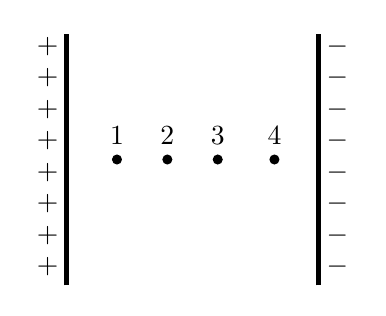
\begin{tikzpicture}[scale=0.8]
    % Musbat plastina (chapda)
    \draw[ultra thick] (0,0) -- (0,4);
    \foreach \y in {0.3, 0.8, ..., 3.8} {
        \node at (-0.3, \y) {$+$};
    }

    % Manfiy plastina (o'ngda)
    \draw[ultra thick] (4,0) -- (4,4);
    
    \foreach \y in {0.3, 0.8, ..., 3.8} {
        \node at (4.3, \y) {$-$};
    }

    % Nuqtalarni belgilash (1, 2, 3, 4)
    % Ular plastinalar orasida bitta gorizontal chiziqda yotadi
    \foreach \x/\n in {0.8/1, 1.6/2, 2.4/3, 3.3/4} {
        \filldraw (\x, 2) circle (2pt) node[above, yshift=2pt] {\n};
    }
    
\end{tikzpicture}

    \begin{enumerate}
    [label=\Alph*)]
        \item $E_1>E_2>E_3>E_4, \quad  \varphi_1=\varphi_2=\varphi_3=\varphi_4$
        \item $E_1<E_2<E_3<E_4, \quad \varphi_1<\varphi_2<\varphi_3<\varphi_4$
        \item $E_1=E_2=E_3=E_4, \quad \varphi_1>\varphi_2>\varphi_3>\varphi_4$
        \item $E_1=E_4>E_2=E_3, \quad \varphi_1=\varphi_4>\varphi_2=\varphi_3$
        \item $E_1<E_2=E_3<E_4, \quad \varphi_1<\varphi_2=\varphi_3<\varphi_4$
    \end{enumerate}

    \item Nuqtaviy musbat zaryadni bir jinsli elektrostatik maydonda O nuqtadan navbat bilan 1-, 2-, 3-, 4- nuqtalarga ko‘chirishda bajarilgan ishlar uchun quyidagi munosabatlarning qaysi biri to‘g‘ri?

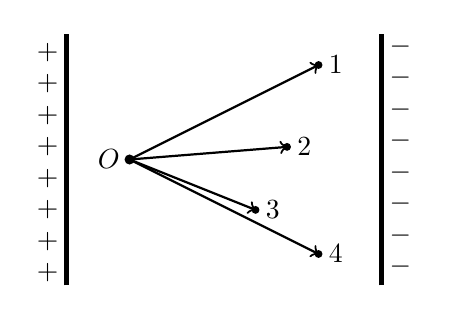
\begin{tikzpicture}[scale=0.8]
    % Chapdagi musbat zaryadlangan plastina
    \draw[ultra thick] (0,0) -- (0,4);
    \foreach \y in {0.2, 0.7, ..., 3.8} {
        \node at (-0.3, \y) {$+$};
    }
    
    \foreach \y in {0.3, 0.8, ..., 3.8} {
        \node at (5.3, \y) {$-$};
    }
    
    % O'ngdagi manfiy zaryadlangan plastina (punktir chiziq bilan)
    \draw[ultra thick] (5,0) -- (5,4);
    

    % O nuqtasi (boshlang'ich holat)
    \coordinate (O) at (1, 2);
    \filldraw (O) circle (2pt) node[left] {$O$};

    % Ko'chish nuqtalari (1, 2, 3, 4)
    % 1, 2 va 4-nuqtalar bir xil gorizontal masofada joylashgan
    \coordinate (P1) at (4, 3.5);
    \coordinate (P2) at (3.5, 2.2);
    \coordinate (P3) at (3, 1.2);
    \coordinate (P4) at (4, 0.5);

    % Yo'nalish strelkalari
    \draw[->, thick] (O) -- (P1) node[right] {1};
    \draw[->, thick] (O) -- (P2) node[right] {2};
    \draw[->, thick] (O) -- (P3) node[right] {3};
    \draw[->, thick] (O) -- (P4) node[right] {4};

    % Nuqtalarning o'zini belgilash
    \foreach \p in {P1, P2, P3, P4} {
        \filldraw (\p) circle (1.5pt);
    }
\end{tikzpicture}

    \begin{enumerate}[label=\Alph*)]
        \item $A_4>A_1>A_2>A_3$
        \item $A_1=A_4>A_2>A_3$
        \item $A_1=A_2=A_3=A_4$
        \item $A_1>A_4>A_2>A_3$
        \item $A_3>A_1=A_2>A_4$
    \end{enumerate}

    \item Biror nuqtaviy zaryaddan qaralayotgan nuqtagacha bo‘lgan masofa 4 marta ortganda zaryad potensiali qanday o‘zgaradi?
    \begin{enumerate}[label=\Alph*)]
        \item 4 marta kamayadi
        \item 4 marta ortadi
        \item 2 marta kamayadi
        \item 2 marta ortadi
        \item 16 marta ortadi
    \end{enumerate}

    \item Nuqtaviy zaryad maydon kuchlanganligi zaryaddan 3,5 cm masofadagi nuqtada 150 V/m bo‘lib, zaryad tomonga yo‘nalgan. Shu nuqtadagi maydon potensiali (V) nimaga teng?
    \begin{enumerate}[label=\Alph*)]
        \item -5,25
        \item -3,75
        \item 3,75
        \item 5,25
        \item 0
    \end{enumerate}

    \item $+q$ hamda $+2q$ nuqtaviy zaryadlar bir biridan $2r$ masofada turibdi. Ularning o‘rtasida joylashgan A nuqtadagi potensial 3 V ga teng. A nuqtadan $2r$ masofaga $Q$ nuqtaviy zaryad joylashtirilganda esa bu nuqtadagi potensial -3 V ni tashkil etdi. $Q$ zaryadni toping.

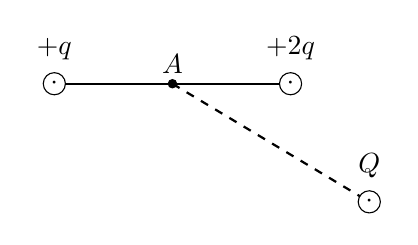
\begin{tikzpicture}[>=stealth, scale=1]
    % Asosiy gorizontal chiziq (+q va +2q orasida)
    \draw[thick] (-1.5,0) -- (1.5,0);

    % +q zaryadi (chapda)
    \filldraw[white, draw=black] (-1.5,0) circle (4pt);
    \node at (-1.5,0) {$\cdot$};
    \node[above, yshift=5pt] at (-1.5,0) {$+q$};

    % +2q zaryadi (o'ngda)
    \filldraw[white, draw=black] (1.5,0) circle (4pt);
    \node at (1.5,0) {$\cdot$};
    \node[above, yshift=5pt] at (1.5,0) {$+2q$};

    % A nuqtasi (o'rtada)
    \filldraw (0,0) circle (1.5pt) node[above] {$A$};

    % Q zaryadigacha bo'lgan punktir chiziq
    % Rasmga ko'ra A dan 2r masofada diagonal pastga yo'nalgan
    \draw[dashed, thick] (0,0) -- (2.5, -1.5);

    % Q zaryadi
    \filldraw[white, draw=black] (2.5,-1.5) circle (4pt);
    \node at (2.5,-1.5) {$\cdot$};
    \node[above, yshift=5pt] at (2.5,-1.5) {$Q$};

\end{tikzpicture}
    
    \begin{enumerate}[label=\Alph*)]
        \item $Q = -12q$
        \item $Q = -6q$
        \item $Q = 6q$
        \item $Q = 12q$
        \item $Q = q$
    \end{enumerate}

    \item $+2q$ va $-q$ zaryadlar rasmdagi kabi o‘rnatilgan. M va N nuqtalar orasidagi potensiallar farqi nimaga teng?

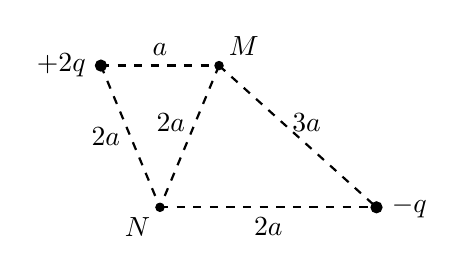
\begin{tikzpicture}[scale=1, >=stealth]
    % Nuqtalar koordinatalari (Rasmga mos nisbatda)
    \coordinate (Q1) at (0, 2);    % +2q zaryadi
    \coordinate (M)  at (1.5, 2);  % M nuqtasi
    \coordinate (N)  at (0.75, 0.2); % N nuqtasi
    \coordinate (Q2) at (3.5, 0.2); % -q zaryadi

    % Masofalarni ko'rsatuvchi punktir chiziqlar va label'lar
    \draw[dashed, thick] (Q1) -- node[above] {$a$} (M);
    \draw[dashed, thick] (Q1) -- node[left] {$2a$} (N);
    \draw[dashed, thick] (M) -- node[left, pos=0.4] {$2a$} (N);
    \draw[dashed, thick] (M) -- node[right, pos=0.4] {$3a$} (Q2);
    \draw[dashed, thick] (N) -- node[below] {$2a$} (Q2);

    % Zaryadlarni va nuqtalarni belgilash
    \filldraw (Q1) circle (2pt) node[left, xshift=-2pt] {$+2q$};
    \filldraw (M)  circle (1.5pt) node[above right] {$M$};
    \filldraw (N)  circle (1.5pt) node[below left] {$N$};
    \filldraw (Q2) circle (2pt) node[right, xshift=2pt] {$-q$};

\end{tikzpicture}
    
    \begin{enumerate}[label=\Alph*)]
        \item $2kq/a$
        \item $2kq/3a$
        \item $3kq/2a$
        \item $7kq/6a$
        \item 0
    \end{enumerate}

    \item $+3q$ va $+4q$ zaryadlar rasmdagi kabi o‘rnatilgan. M va N nuqtalar orasidagi potensiallar farqi nimaga teng?

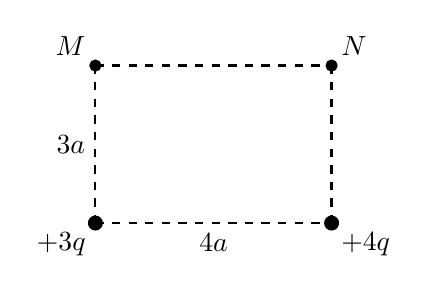
\begin{tikzpicture}
    % Nuqtalar koordinatalari
    \coordinate (M) at (0, 2);    % Yuqori chap nuqta
    \coordinate (N) at (3, 2);    % Yuqori o'ng nuqta
    \coordinate (Q1) at (0, 0);   % Pastki chap (+3q)
    \coordinate (Q2) at (3, 0);   % Pastki o'ng (+4q)

    % To'rtburchak tomonlarini ko'rsatuvchi punktir chiziqlar va masofalar
    \draw[dashed, thick] (M) -- node[left] {$3a$} (Q1);
    \draw[dashed, thick] (M) -- (N);
    \draw[dashed, thick] (N) -- (Q2);
    \draw[dashed, thick] (Q1) -- node[below] {$4a$} (Q2);

    % Nuqtalarni belgilash (M va N)
    \filldraw (M) circle (2pt) node[above left] {$M$};
    \filldraw (N) circle (2pt) node[above right] {$N$};

    % Zaryadlarni belgilash (+3q va +4q)
    \filldraw (Q1) circle (2.5pt) node[below left] {$+3q$};
    \filldraw (Q2) circle (2.5pt) node[below right] {$+4q$};

\end{tikzpicture}
    
    \begin{enumerate}[label=\Alph*)]
        \item $kq/15a$
        \item $2kq/15a$
        \item $kq/5a$
        \item $4kq/15a$
        \item $kq/3a$
    \end{enumerate}

    \item Rasmdagi to‘rtta zaryadning O nuqtadagi natijaviy elektr maydon kuchlanganligi 25 V/m ga teng bo‘lsa, shu nuqtadagi natijaviy potensiali necha Volt?

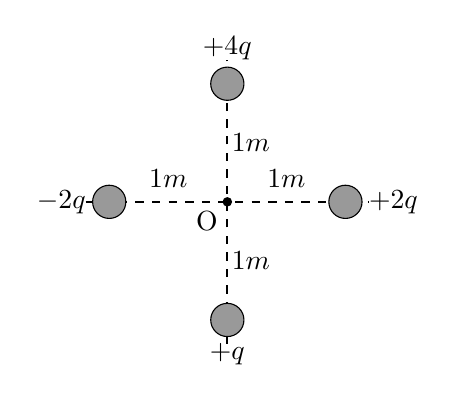
\begin{tikzpicture}[scale=1.5, >=stealth]
    % Koordinata o'qlari (punktir chiziqlar)
    \draw[dashed, thick] (0,-1.2) -- (0,1.2);
    \draw[dashed, thick] (-1.2,0) -- (1.2,0);

    % Markaziy O nuqtasi
    \filldraw (0,0) circle (1pt) node[below left] {O};
    
    \filldraw (0,0) circle (0.5pt);

    % Zaryadlarni joylashtirish va belgilash
    % Yuqorida +4q
    \filldraw[gray!80, draw=black] (0,1) circle (4pt) node[above, yshift=5pt, black] { $+4q$};
    % Pastda +q
    \filldraw[gray!80, draw=black] (0,-1) circle (4pt) node[below, yshift=-5pt, black] { $+q$};
    % Chapda -2q
    \filldraw[gray!80, draw=black] (-1,0) circle (4pt) node[left, xshift=-5pt, black] { $-2q$};
    % O'ngda +2q
    \filldraw[gray!80, draw=black] (1,0) circle (4pt) node[right, xshift=5pt, black] { $+2q$};

    % Masofalarni ko'rsatuvchi yozuvlar (1 m)
    \node at (0.2, 0.5) { $1\text{ m}$};
    \node at (0.2, -0.5) { $1\text{ m}$};
    \node at (-0.5, 0.2) { $1\text{ m}$};
    \node at (0.5, 0.2) { $1\text{ m}$};

\end{tikzpicture}
    
    \begin{enumerate}[label=\Alph*)]
        \item 25
        \item 30
        \item 35
        \item 40
        \item 50
    \end{enumerate}

    \item Radiuslari $R_1=R$ va $R_2=2R$ bo‘lgan metall sharlardagi zaryadning sirt zichligi bir xil. Sharlar markazlari-dagi potensiallarni solishtiring.
    \begin{enumerate}[label=\Alph*)]
        \item $\varphi_2=2\varphi_1$
        \item $\varphi_1=2\varphi_2$
        \item $\varphi_1=\varphi_2$
        \item $\varphi_1=4\varphi_2$
        \item $\varphi_2=4\varphi_1$
    \end{enumerate}

    \item Radiusi 10 cm va potensiali 200 V bo‘lgan zaryadlangan o‘tkazuvchi sfera markazidagi kuchlanganlik va potensial nimaga teng?
    \begin{enumerate}[label=\Alph*)]
        \item 0; 0
        \item 200 V/m; 200 V
        \item 200 V/m; 0
        \item 10 V/m; 100 V
        \item 0; 200 V
    \end{enumerate}

    \item Potensiali va radiusi rasmda ko‘rsatilgan x va y sharlar bir-biriga tekkizildi. Shundan so‘ng sharlarning potensiali nimaga teng bo‘lib qoladi?

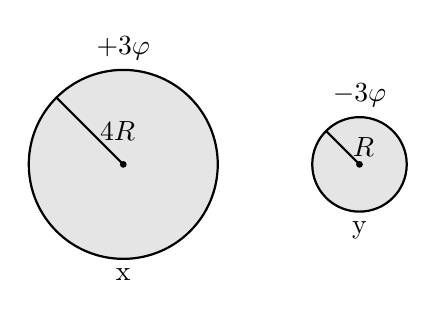
\begin{tikzpicture}[scale=1, >=stealth]
    % x shari (kattaroq)
    \draw[thick, fill=gray!20] (0,0) circle (1.2); % Radiusi 4R ni ifodalash uchun
    \filldraw (0,0) circle (1pt); % Markazi
    \draw[thick] (0,0) -- (-0.85, 0.85) node[midway, right] { $4R$}; % Radius chizig'i
    \node[above] at (0, 1.2) { $+3\varphi$}; % Potensiali
    \node[below] at (0, -1.2) {x}; % Shar nomi

    % y shari (kichikroq)
    \draw[thick, fill=gray!20] (3,0) circle (0.6); % Radiusi R ni ifodalash uchun
    \filldraw (3,0) circle (1pt); % Markazi
    \draw[thick] (3,0) -- (2.57, 0.43) node[midway, right] { $R$}; % Radius chizig'i
    \node[above] at (3, 0.6) {$-3\varphi$}; % Potensiali
    \node[below] at (3, -0.6) {y}; % Shar nomi

\end{tikzpicture}
    
    \begin{enumerate}[label=\Alph*)]
        \item 0
        \item $-2\varphi/3$
        \item $+\varphi$
        \item $+9\varphi/5$
        \item $+2\varphi$
    \end{enumerate}

    \item Rasmdagi K shar avval L sharga, keyin M sharga tekkizib olindi. Shundan so‘ng sharlarning zaryadi nimaga teng bo‘lib qoladi?

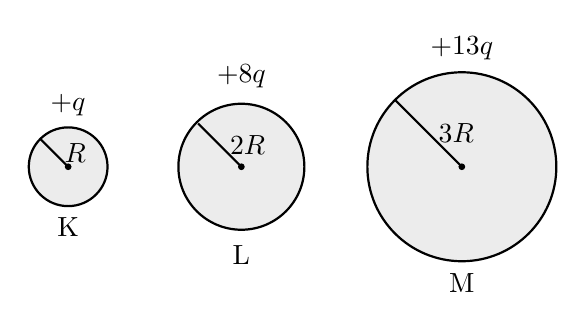
\begin{tikzpicture}[scale=1, >=stealth]
    % K shari (eng kichigi)
    \draw[thick, fill=gray!15] (0,0) circle (0.5); 
    \filldraw (0,0) circle (1pt); % Markazi
    \draw[thick] (0,0) -- (-0.35, 0.35) node[midway, right] {$R$}; % Radiusi
    \node[above, yshift=15pt] at (0,0) {$+q$}; % Zaryadi
    \node[below, yshift=-15pt] at (0,0) {K}; % Nomi

    % L shari (o'rtacha)
    \draw[thick, fill=gray!15] (2.2,0) circle (0.8); 
    \filldraw (2.2,0) circle (1pt); % Markazi
    \draw[thick] (2.2,0) -- (1.65, 0.55) node[midway, right] {$2R$}; % Radiusi
    \node[above, yshift=25pt] at (2.2,0) {$+8q$}; % Zaryadi
    \node[below, yshift=-25pt] at (2.2,0) {L}; % Nomi

    % M shari (eng kattasi)
    \draw[thick, fill=gray!15] (5,0) circle (1.2); 
    \filldraw (5,0) circle (1pt); % Markazi
    \draw[thick] (5,0) -- (4.15, 0.85) node[midway, right] {$3R$}; % Radiusi
    \node[above, yshift=35pt] at (5,0) {$+13q$}; % Zaryadi
    \node[below, yshift=-35pt] at (5,0) {M}; % Nomi

\end{tikzpicture}
    
    \begin{enumerate}[label=\Alph*)]
        \item $+q; +18q; +3q$
        \item $+6q; +q; +18q$
        \item $+4q; +6q; +12q$
        \item $+10q; +4q; +8q$
        \item $+2q; +12q; +6q$
    \end{enumerate}

    \item Rasmdagi K shar avval L sharga, keyin M sharga tekkizib olindi. Shundan so‘ng L sharning zaryadi nimaga teng bo‘lib qoladi?

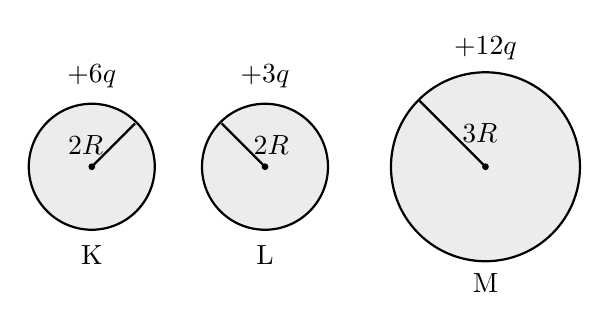
\begin{tikzpicture}[scale=1, >=stealth]
    % K shari (eng kichigi)
   \draw[thick, fill=gray!15] (0,0) circle (0.8); 
    \filldraw (0,0) circle (1pt); % Markazi
    \draw[thick] (0,0) -- (0.55, 0.55) node[midway, left] {$2R$}; % Radiusi
    \node[above, yshift=25pt] at (0,0) {$+6q$}; % Zaryadi
    \node[below, yshift=-25pt] at (0,0) {K}; % Nomi

    % L shari (o'rtacha)
    \draw[thick, fill=gray!15] (2.2,0) circle (0.8); 
    \filldraw (2.2,0) circle (1pt); % Markazi
    \draw[thick] (2.2,0) -- (1.65, 0.55) node[midway, right] {$2R$}; % Radiusi
    \node[above, yshift=25pt] at (2.2,0) {$+3q$}; % Zaryadi
    \node[below, yshift=-25pt] at (2.2,0) {L}; % Nomi

    % M shari (eng kattasi)
    \draw[thick, fill=gray!15] (5,0) circle (1.2); 
    \filldraw (5,0) circle (1pt); % Markazi
    \draw[thick] (5,0) -- (4.15, 0.85) node[midway, right] {$3R$}; % Radiusi
    \node[above, yshift=35pt] at (5,0) {$+12q$}; % Zaryadi
    \node[below, yshift=-35pt] at (5,0) {M}; % Nomi

\end{tikzpicture}
    
    \begin{enumerate}[label=\Alph*)]
        \item $+q$
        \item $+3q$
        \item $+2q$
        \item $+6q$
        \item $+5q$
    \end{enumerate}

\end{enumerate}